% !TEX root = SystemTemplate.tex

\chapter{User Documentation}

This section will contain the basis for any end user documentation for the system, 
and will cover the basic steps for the setup and use of the system.



\section{User Guide}
Usage of the Auto Tester is primarily concerned with the format and placement of the test case files. 
Test case files must be located in the same directory as the students program source, or in a subdirectory 
there of. The golden cpp, if present, must be given in the commandline, or be located in the first directory given.

\subsection{Test Case Files}
Files that contain the test cases themselves need to be given a .tst extension. The filname proceeding the 
extension will be used as the name of that test in the log file. The contents of the file will be the raw 
input to the student's program.

\subsection{Expected Output Files}
For each test case file, there needs to be a corresponding file that contains the expected output. This file 
must have the same name as the test case, but instead have a .ans extension.

\subsection{Auto Generated Tests}
The option to auto generate tests with a given 'golden cpp' will be available to the user. The user will run 
the Auto Tester with a given program, and then will go through a simple text based menu that will determine the 
parameters for the auto generated tests. The code will then place the .tst and .ans files in a subdirectory called "tests". The answer files will be generated by running the test files through the golden cpp.

\subsection{Results}
The results for each student will be placed in a file with a .log extension, within the given student's directory. 
In addition, a complete log with the names of all the students and their pass/fail status and/or grade will be placed 
in the head directory. The filenames will be timestamped. Gcov information is put in each student log file. Gprof information is put in the student directory with the naming convention [time stamp]profile.out.

\begin{figure}[H]
\begin{center}
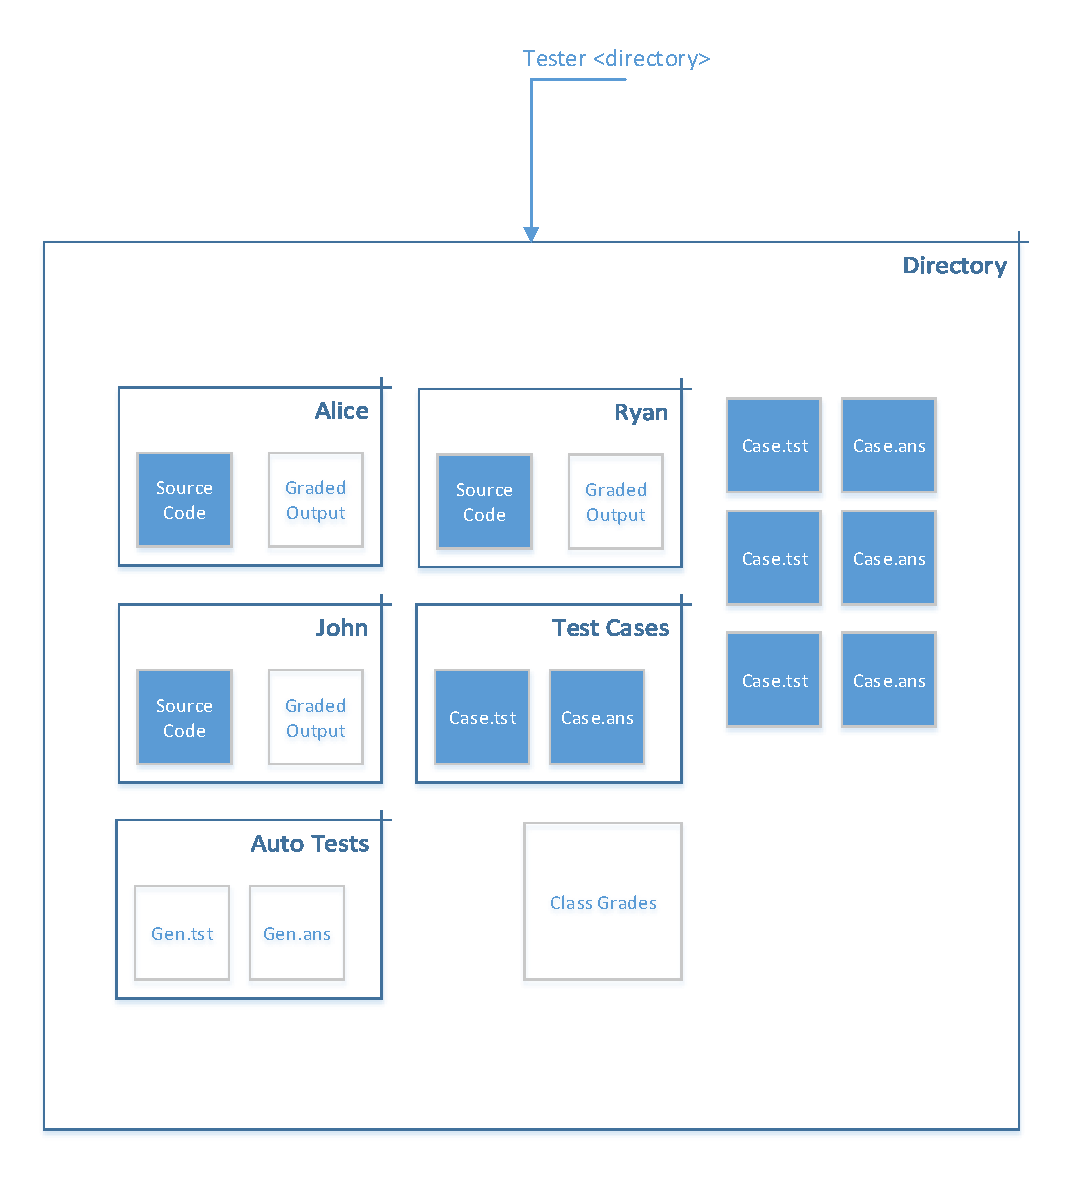
\includegraphics[width=0.75\textwidth]{./Dir_struct}
\end{center}
\caption{Example directory structure for runnning the tester \label{dir}}
\end{figure}

\section{Installation Guide}
To use the application, compile the source code using the supplied makefile.

After this is completed, the user should have an
executable file they can use by invoking the following: \\
./tester [-g or -r] $\langle$ directory $\rangle$ [-p or empty]

\section{Programmer Manual}
The code contained in the .cpp file is written in c++ and is to be compiled with g++.
